\documentclass[11pt, a4paper]{article}

\usepackage{graphicx}
\usepackage[english]{babel}
\usepackage[utf8x]{inputenc}
\usepackage{amsmath}
\usepackage[a4paper,top=3cm,bottom=2cm,left=2cm,right=2cm,marginparwidth=1.75cm]{geometry}
\usepackage{amssymb}
\usepackage{subfig}

\graphicspath{ {./images} }
\newcommand*{\qed}{\hfill\ensuremath{\quad\square}}%
\newcommand*{\rad}{\ensuremath{\,\text{rad}}}
\newcommand*{\R}{\ensuremath{\mathbb{R}}}

\makeatletter
\renewcommand*\env@matrix[1][*\c@MaxMatrixCols c]{%
  \hskip -\arraycolsep
  \let\@ifnextchar\new@ifnextchar
  \array{#1}}
\makeatother

\newtheorem{theorem}{Theorem}

%------------------------------------------------
%Templates for images and figures
% \begin{figure}[h]
%   \centering
%   \subfloat[caption 1]{{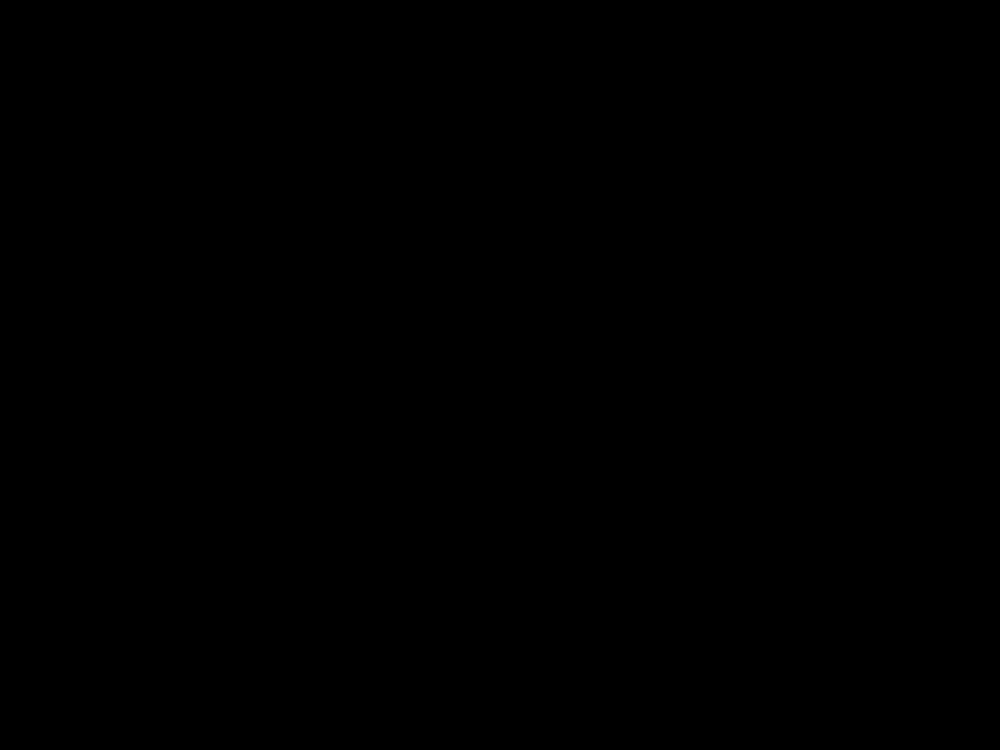
\includegraphics[width=30mm]{images/placeholder.png}}}%
%   \qquad
%   \subfloat[caption 2]{{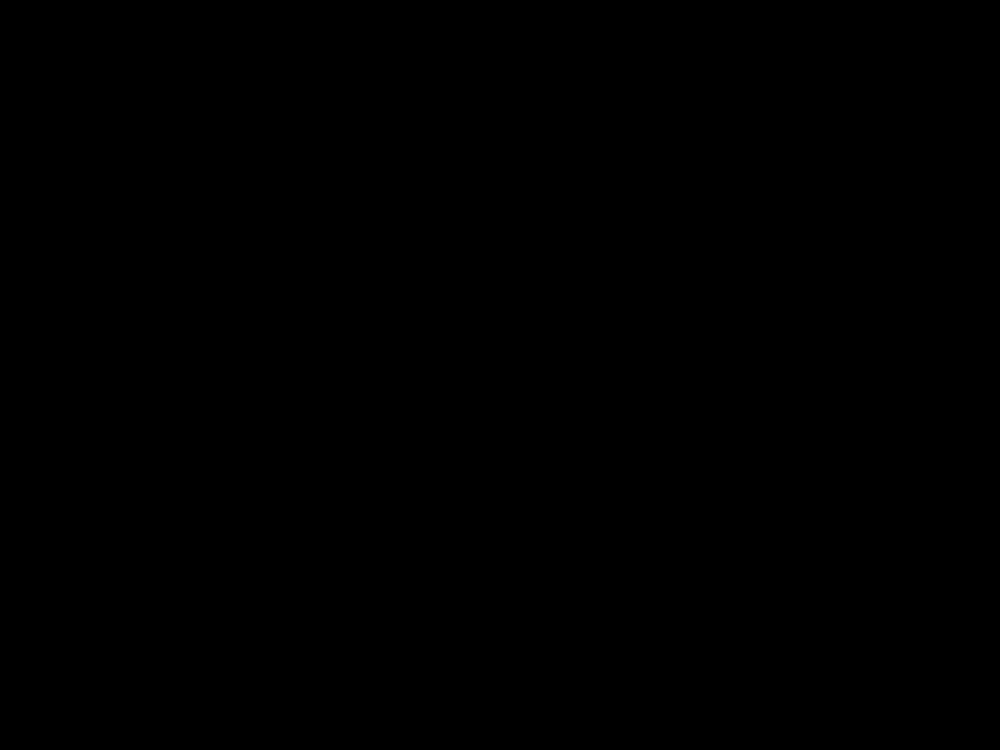
\includegraphics[width=30mm]{images/placeholder.png}}}%
%   \caption{Description}
% \end{figure}

% \begin{figure}[h]
%   \centerline{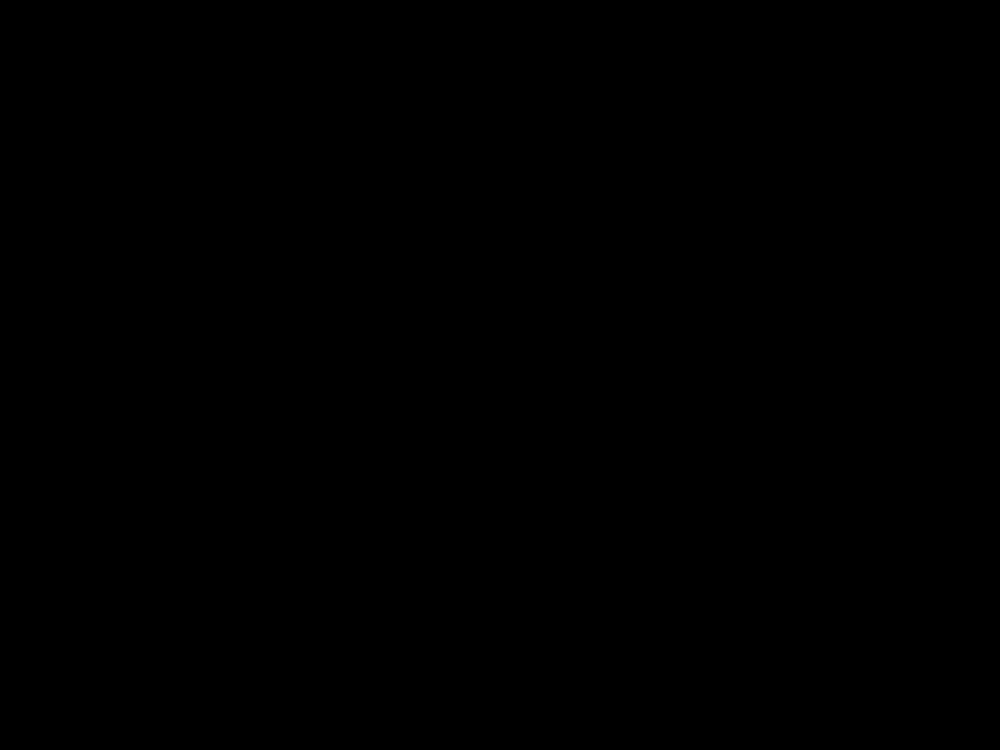
\includegraphics[width=50mm]{images/placeholder.png}}
%   \caption{Description}
% \end{figure}
%-----------------------------------------------

\begin{document}

\setcounter{section}{12}
\section{Lecture 13: The Gram-Schmidt process (24/03/2020)}
\subsection{The Gram-Schmidt process}
The Gram-Schmidt process is a simple process that can take any random basis for a subspace $W$, and produces and orthogonal or orthonormal basis for any random subspace of $\R^n$.

\begin{theorem}
  Given a basis $\{\vec{x}_1, \cdots, \vec{x}_p \}$ for a non-zero subspace $W$ of $\R^n$ define:
  \begin{align*}
    \vec{v}_1 &= \vec{x}_1\\
    \vec{v}_2 &= \vec{x}_2 - \frac{\langle \vec{x}_2 | \vec{v}_1 \rangle}{\langle \vec{v}_1 | \vec{v}_1 \rangle}\vec{v}_1\\
    \vec{v}_3 &= \vec{x}_3 - \frac{\langle \vec{x}_3 | \vec{v}_1 \rangle}{\langle \vec{v}_1 | \vec{v}_1 \rangle}\vec{v}_1 - \frac{\langle \vec{x}_3 | \vec{v}_2 \rangle}{\langle \vec{v}_2 | \vec{v}_2 \rangle}\vec{v}_2\\
    &\vdots\\
    \vec{v}_p &= \vec{x}_p - \frac{\langle \vec{x}_p | \vec{v}_1 \rangle}{\langle \vec{v}_1 | \vec{v}_1 \rangle}\vec{v}_1 - \frac{\langle \vec{x}_p | \vec{v}_2 \rangle}{\langle \vec{v}_2 | \vec{v}_2 \rangle}\vec{v}_2 - \cdots - \frac{\langle \vec{x}_p | \vec{v}_{p-1} \rangle}{\langle \vec{v}_{p-1} | \vec{v}_{p-1} \rangle}\vec{v}_{p-1}
  \end{align*}
  Then $\{\vec{v}_1, \cdots, \vec{v}_p \}$ is an orthogonal basis for $W$. In addition $\text{Span}\{\vec{v}_1, \cdots, \vec{v}_k\} = \text{Span}\{\vec{x}_1, \cdots, \vec{x}_k \}$ for $1 \leq k \leq p$
\end{theorem}

\subsection{Orthonormal Basis from the Gram-Schmidt process}
The basis found from the Gram-Schmidt process in theorem 1 can be normalized to obtain an orthonormal basis.
\begin{gather}
  \text{orthogonal basis: } \{\vec{v}_1, \cdots, \vec{v}_p\} \notag\\
  \text{orthonormal basis: } \{\vec{u}_1, \cdots, \vec{u}_p\} \notag\\
  \vec{u}_i = \frac{\vec{v}_i}{||\vec{v}_i||}
\end{gather}


\end{document}